\documentclass[aspectratio=169,10pt]{beamer}

\usetheme{Madrid}
\usecolortheme{seahorse}

\usepackage{amsmath,amssymb}
\usepackage{booktabs}
\usepackage{array}
\usepackage{graphicx}
\usepackage{listings}
\usepackage{ragged2e}
\usepackage{tabularx}
\usepackage{tikz}
\usepackage{pgfplots}
\usepackage{iftex}
\pgfplotsset{compat=1.18}

\ifPDFTeX
  \pdfmapfile{+cm.map}
  \pdfmapfile{+cmextra.map}
  \pdfmapfile{+symbols.map}
\fi

\definecolor{CourseBlue}{RGB}{41,77,115}
\definecolor{CourseGreen}{RGB}{63,125,88}
\definecolor{CourseGold}{RGB}{190,137,45}
\definecolor{CourseRed}{RGB}{169,75,70}
\definecolor{SoftGrid}{RGB}{218,225,232}
\definecolor{CodeBack}{RGB}{245,247,249}

\setbeamercolor{structure}{fg=CourseBlue}
\setbeamertemplate{navigation symbols}{}
\setbeamertemplate{itemize items}[circle]
\setbeamertemplate{enumerate items}[default]

\lstdefinestyle{Rstyle}{
  language=R,
  basicstyle=\ttfamily\scriptsize,
  keywordstyle=\color{CourseBlue}\bfseries,
  commentstyle=\color{CourseGreen!80!black},
  stringstyle=\color{CourseRed!85!black},
  backgroundcolor=\color{CodeBack},
  frame=single,
  rulecolor=\color{SoftGrid},
  showstringspaces=false,
  breaklines=true,
  columns=fullflexible,
  keepspaces=true
}

\title[Chapter 19: Inference about a Proportion]{\textbf{Chapter 19: Inference about a Population Proportion}}
\subtitle{The Practice of Statistics in the Life Sciences \\ Brigitte Baldi and David S. Moore}
\author{Instructor: Ali Raisolsadat}
\date{Part IV: Specific Inference Procedures}

\begin{document}

% SLIDE 1
\begin{frame}
  \titlepage
\end{frame}

% SLIDE 2
\begin{frame}{Why Chapter 19 Matters}
Earlier chapters developed inference for population means using quantitative data.

\vspace{0.25cm}
Many scientific questions instead record a categorical outcome with two possible categories.

\begin{itemize}
  \item Does a person currently test positive for an infection?
  \item Does a patient respond to treatment?
  \item Does an animal display a particular behaviour?
\end{itemize}

\begin{block}{Main Question}
How can a sample proportion be used to estimate or test an unknown population proportion?
\end{block}
\end{frame}

% SLIDE 3
\begin{frame}{Chapter Roadmap}
The chapter develops five connected ideas.

\begin{enumerate}
  \item The sample proportion and its sampling distribution
  \item Large-sample confidence intervals
  \item The more accurate plus four confidence interval
  \item Sample-size planning for a desired margin of error
  \item One-proportion hypothesis tests
\end{enumerate}

\vspace{0.2cm}
The theory comes first. Each procedure is then applied to a life-science example and reproduced in R.
\end{frame}

% SLIDE 4
\begin{frame}{Means and Proportions}
\begin{center}
\begin{tabularx}{0.94\textwidth}{>{\RaggedRight\arraybackslash}p{0.25\textwidth} X X}
\toprule
 & \textbf{Quantitative response} & \textbf{Binary categorical response} \\
\midrule
Population parameter & Mean $\mu$ & Proportion $p$ \\
Sample statistic & Mean $\bar{x}$ & Proportion $\hat{p}$ \\
Typical question & Average measurement & Fraction with an outcome \\
Reference model & $t$ or Normal & Approximately Normal \\
\bottomrule
\end{tabularx}
\end{center}

The inferential logic remains the same: use a sample statistic to learn about an unknown population parameter while accounting for sampling variation.
\end{frame}

% SLIDE 5
\begin{frame}{Defining the Outcome}
For convenience, the outcome being counted is called a \textbf{success}. The label does not imply that the outcome is desirable.

\vspace{0.2cm}
Before collecting or analyzing data, define

\begin{itemize}
  \item The target population
  \item The observational unit
  \item The exact rule that identifies a success
  \item The time period or measurement window
\end{itemize}

\begin{block}{Why the Definition Matters}
Different definitions of \emph{smoker}, \emph{infection} or \emph{treatment response} can produce very different proportions from the same population.
\end{block}
\end{frame}

% SLIDE 6
\begin{frame}{The Sample Proportion}
Suppose a sample contains $n$ individuals and $X$ successes.

\begin{block}{Sample Proportion}
\[
\hat{p}=\frac{X}{n}
\]
\end{block}

The statistic $\hat{p}$ estimates the unknown population proportion $p$.

\begin{itemize}
  \item $\hat{p}$ is read as \emph{p-hat}
  \item $0\leq\hat{p}\leq1$
  \item $100\hat{p}\%$ is the corresponding sample percentage
  \item A different random sample usually produces a different value of $\hat{p}$
\end{itemize}
\end{frame}

% SLIDE 7
\begin{frame}{Example 19.1: HPV Prevalence}
A nationally representative survey obtained valid specimens from $1921$ women aged $14$ to $59$. Of these specimens, $515$ tested positive for HPV.

\begin{block}{Sample Estimate}
\[
\hat{p}=\frac{515}{1921}\approx0.2681
\]
\[
100\hat{p}\%\approx26.81\%
\]
\end{block}

The observed percentage describes the sample. Inference is needed to estimate the proportion $p$ of all women in the target population who would test positive.
\end{frame}

% SLIDE 8
\begin{frame}{Sampling Distribution of $\hat{p}$}
For a random sample of size $n$ from a large population with proportion $p$,

\textbf{Centre}
\[
\mu_{\hat{p}}=p
\]

\textbf{Spread}
\[
\sigma_{\hat{p}}=\sqrt{\frac{p(1-p)}{n}}
\]

The sample proportion is an unbiased estimator of $p$. Its sampling variability decreases as the sample size increases.
\end{frame}

% SLIDE 9
\begin{frame}{Shape of the Sampling Distribution}
When the expected numbers of successes and failures are sufficiently large, the sampling distribution of $\hat{p}$ is approximately Normal.

\begin{center}
\begin{tikzpicture}
\begin{axis}[
  width=0.82\textwidth,
  height=0.48\textheight,
  axis lines=left,
  xmin=0.20,xmax=0.34,
  ymin=0,ymax=42,
  xtick={0.20,0.22,0.24,0.26,0.28,0.30,0.32,0.34},
  ytick=\empty,
  xlabel={Possible values of $\hat{p}$},
  ylabel={Density},
  grid=major,
  grid style={SoftGrid,dotted}
]
\addplot[CourseBlue,very thick,domain=0.20:0.34,samples=180]
{1/(0.0101*sqrt(2*pi))*exp(-((x-0.2681)^2)/(2*0.0101^2))};
\addplot[CourseRed,dashed,thick] coordinates {(0.2681,0) (0.2681,40)};
\end{axis}
\end{tikzpicture}
\end{center}

The approximation can be poor when $n$ is small or when $p$ is close to $0$ or $1$.
\end{frame}

% SLIDE 10
\begin{frame}{Conditions for Inference about a Proportion}
Inference about one population proportion requires three ideas.

\begin{itemize}
  \item \textbf{Randomness:} The data can be treated as a simple random sample or arise from another defensible random process
  \item \textbf{Independence:} The population is much larger than the sample, often checked with $n\leq0.10N$
  \item \textbf{Large counts:} The relevant procedure has enough expected or observed successes and failures for its Normal approximation
\end{itemize}

\begin{block}{Design Before Formula}
A larger sample reduces random sampling error. It does not remove selection bias, nonresponse bias or an unclear definition of success.
\end{block}
\end{frame}


% SLIDE 11
\begin{frame}{Anatomy of a Confidence Interval}
A confidence interval for a population proportion has the familiar form

\[
\text{estimate}\pm\text{critical value}\times\text{standard error}
\]

Using $\hat{p}$ to estimate $p$ gives

\[
SE_{\hat{p}}=\sqrt{\frac{\hat{p}(1-\hat{p})}{n}}
\]

The margin of error is

\[
m=z^*SE_{\hat{p}}
\]

The critical value $z^*$ comes from the Standard Normal distribution.
\end{frame}

% SLIDE 12
\begin{frame}{Large-Sample Confidence Interval}
For a random sample from a large population, the approximate level $C$ interval is

\begin{block}{Large-Sample Interval}
\[
\hat{p}\pm z^*\sqrt{\frac{\hat{p}(1-\hat{p})}{n}}
\]
\end{block}

Common critical values are

\begin{center}
\begin{tabular}{cc}
\toprule
Confidence level & $z^*$ \\
\midrule
$90\%$ & $1.645$ \\
$95\%$ & $1.960$ \\
$99\%$ & $2.576$ \\
\bottomrule
\end{tabular}
\end{center}
\end{frame}

% SLIDE 13
\begin{frame}{Why the Critical Value Is $z^*$}
Inference for a mean uses a $t$ distribution when the separate spread parameter $\sigma$ must be estimated by $s$.

\vspace{0.2cm}
For a proportion, the sampling variance is determined by the same parameter being estimated:

\[
\operatorname{Var}(\hat{p})=\frac{p(1-p)}{n}
\]

Replacing $p$ with $\hat{p}$ does not create a $t$ statistic. The method continues to use a Normal approximation and a $z^*$ critical value.
\end{frame}

% SLIDE 14
\begin{frame}{Conditions for the Large-Sample Interval}
Use the ordinary large-sample interval only when

\begin{itemize}
  \item The sampling design supports inference to the target population
  \item The population is much larger than the sample
  \item The sample contains at least $15$ successes
  \item The sample contains at least $15$ failures
\end{itemize}

\[
X\geq15
\qquad\text{and}\qquad
n-X\geq15
\]

Observed counts are used because the population proportion $p$ is unknown.
\end{frame}

% SLIDE 15
\begin{frame}{Example 19.3: HPV Confidence Interval}
\begin{block}{State}
Estimate the proportion $p$ of women aged $14$ to $59$ in the target population who currently test positive for HPV.
\end{block}

\begin{block}{Plan}
Construct a $95\%$ large-sample confidence interval using $X=515$ positive specimens from $n=1921$ valid specimens.
\end{block}

The point estimate is

\[
\hat{p}=\frac{515}{1921}=0.2681
\]
\end{frame}

% SLIDE 16
\begin{frame}{Example 19.3: Checking the Conditions}
\begin{itemize}
  \item NHANES used a complex representative sampling design. The analysis treats its overall behaviour as approximately comparable to an SRS
  \item The target population is much larger than $1921$
  \item The number of successes is $515$
  \item The number of failures is $1921-515=1406$
\end{itemize}

\[
515\geq15
\qquad\text{and}\qquad
1406\geq15
\]

The count condition is easily satisfied. The sampling design requires more careful interpretation than the calculation alone suggests.
\end{frame}

% SLIDE 17
\begin{frame}{Example 19.3: Calculating the Interval}
The estimated standard error is

\[
SE=\sqrt{\frac{(0.2681)(0.7319)}{1921}}\approx0.01011
\]

The margin of error is

\[
m=1.960(0.01011)\approx0.01981
\]

The $95\%$ confidence interval is

\[
0.2681\pm0.01981
\]

\[
\boxed{(0.2483,\ 0.2879)}
\]
\end{frame}

% SLIDE 18
\begin{frame}[fragile]{Example 19.3: Calculation in R}
\begin{lstlisting}[style=Rstyle]
# Observed count and sample size
x_hpv <- 515
n_hpv <- 1921

# Large-sample 95% confidence interval
p_hat_hpv <- x_hpv / n_hpv
se_hpv <- sqrt(p_hat_hpv * (1 - p_hat_hpv) / n_hpv)
z_star <- qnorm(0.975)
margin_hpv <- z_star * se_hpv

c(
  estimate = p_hat_hpv,
  lower = p_hat_hpv - margin_hpv,
  upper = p_hat_hpv + margin_hpv
)
\end{lstlisting}
\end{frame}

% SLIDE 19
\begin{frame}{Example 19.3: Interpretation and Scope}
We are $95\%$ confident that the proportion of women aged $14$ to $59$ in the target population who would currently test positive for HPV lies between approximately $0.248$ and $0.288$.

\vspace{0.2cm}
Equivalently, the estimated population percentage is between approximately $24.8\%$ and $28.8\%$.

\begin{block}{Study Limitation}
About $23\%$ of the original sample did not provide a usable specimen. If respondents and nonrespondents differ in HPV prevalence, nonresponse can bias the estimate. The margin of error does not measure that bias.
\end{block}
\end{frame}

% SLIDE 20
\begin{frame}{Limitations of the Ordinary Interval}
The large-sample interval is easy to calculate, but its actual coverage can fall below the requested confidence level.

\vspace{0.2cm}
Problems are most noticeable when

\begin{itemize}
  \item The sample size is modest
  \item The number of successes is small
  \item The number of failures is small
  \item The true population proportion is close to $0$ or $1$
\end{itemize}

A simple adjustment improves coverage substantially in many of these settings.
\end{frame}


% SLIDE 21
\begin{frame}{The Plus Four Method}
The plus four method adds four imaginary observations:

\begin{itemize}
  \item Two successes
  \item Two failures
\end{itemize}

The adjusted estimate is

\begin{block}{Plus Four Estimate}
\[
\widetilde{p}=\frac{X+2}{n+4}
\]
\end{block}

The confidence interval then uses the ordinary formula with $\widetilde{p}$ and the adjusted sample size $n+4$.
\end{frame}

% SLIDE 22
\begin{frame}{Plus Four Confidence Interval}
The plus four interval is

\[
\widetilde{p}
\pm
z^*
\sqrt{
\frac{
\widetilde{p}(1-\widetilde{p})
}{
n+4
}
}
\]

Use this method when

\begin{itemize}
  \item The confidence level is at least $90\%$
  \item The original sample size satisfies $n\geq10$
  \item The sampling and independence conditions are reasonable
\end{itemize}

The adjustment moves the estimate slightly toward $0.5$, where the Normal approximation behaves more reliably.
\end{frame}

% SLIDE 23
\begin{frame}{Example 19.4: Blinding in Clinical Trials}
Investigators randomly selected $97$ articles that reported placebo-controlled clinical trials. Only $7$ articles discussed whether blinding had succeeded.

\begin{block}{Question}
What proportion $p$ of all similar articles discuss the success of blinding?
\end{block}

The ordinary large-sample interval is not recommended because the sample contains only $7$ successes. The sample size is large enough for a plus four interval.
\end{frame}

% SLIDE 24
\begin{frame}{Example 19.4: Plus Four Calculation}
The adjusted estimate is

\[
\widetilde{p}
=
\frac{7+2}{97+4}
=
\frac{9}{101}
\approx0.0891
\]

The adjusted standard error is

\[
SE
=
\sqrt{\frac{(0.0891)(0.9109)}{101}}
\approx0.02835
\]

The $95\%$ plus four interval is

\[
0.0891\pm1.960(0.02835)
=
\boxed{(0.0335,\ 0.1447)}
\]
\end{frame}

% SLIDE 25
\begin{frame}[fragile]{Example 19.4: Plus Four Interval in R}
\begin{lstlisting}[style=Rstyle]
# Original study results
x_blind <- 7
n_blind <- 97

# Add two successes and two failures
x_plus4 <- x_blind + 2
n_plus4 <- n_blind + 4
p_plus4 <- x_plus4 / n_plus4

se_plus4 <- sqrt(p_plus4 * (1 - p_plus4) / n_plus4)
margin_plus4 <- qnorm(0.975) * se_plus4

c(
  estimate = p_plus4,
  lower = p_plus4 - margin_plus4,
  upper = p_plus4 + margin_plus4
)
\end{lstlisting}
\end{frame}

% SLIDE 26
\begin{frame}{Ordinary and Plus Four Intervals}
For the blinding example,

\begin{center}
\begin{tabular}{lccc}
\toprule
Method & Estimate & Lower bound & Upper bound \\
\midrule
Ordinary large-sample & $0.0722$ & $0.0207$ & $0.1237$ \\
Plus four & $0.0891$ & $0.0335$ & $0.1447$ \\
\bottomrule
\end{tabular}
\end{center}

The numerical difference is modest, but the repeated-sampling coverage of the plus four method is more reliable.

\begin{block}{Recommended Method}
Use the plus four interval when estimating one population proportion under its stated conditions.
\end{block}
\end{frame}

% SLIDE 27
\begin{frame}{Choosing a Sample Size}
To plan for a margin of error no greater than $m$, use

\begin{block}{Required Sample Size}
\[
n
=
\left(\frac{z^*}{m}\right)^2
p^*(1-p^*)
\]
\end{block}

Here, $p^*$ is a planning value for the anticipated population proportion.

\vspace{0.2cm}
Always round the calculated sample size \textbf{up}. Rounding down can produce a margin of error larger than requested.
\end{frame}

% SLIDE 28
\begin{frame}{Choosing the Planning Value $p^*$}
Two approaches are common.

\begin{itemize}
  \item Use a value from a pilot study, previous research or credible subject-matter knowledge
  \item Use $p^*=0.5$ when no useful prior estimate is available
\end{itemize}

The product $p^*(1-p^*)$ is largest at $p^*=0.5$:

\[
(0.5)(1-0.5)=0.25
\]

This choice gives the largest required sample size and therefore provides a conservative plan.
\end{frame}

% SLIDE 29
\begin{frame}{Example 19.5: Planning a Survey}
A university wants to estimate the proportion of students who never floss. The desired confidence level is $95\%$, and the margin of error should be no greater than $0.04$.

\vspace{0.2cm}
With no precise prior estimate, use $p^*=0.5$:

\[
n
=
\left(\frac{1.960}{0.04}\right)^2
(0.5)(0.5)
=
600.25
\]

Round upward:

\[
\boxed{n=601}
\]
\end{frame}

% SLIDE 30
\begin{frame}[fragile]{Sample-Size Planning in R}
\begin{lstlisting}[style=Rstyle]
# Desired design values
confidence <- 0.95
margin <- 0.04
p_star <- 0.50

# Critical value and required sample size
z_star <- qnorm(1 - (1 - confidence) / 2)
n_required <- (z_star / margin)^2 *
  p_star * (1 - p_star)

ceiling(n_required)
# [1] 601
\end{lstlisting}

For margins of error $0.03$ and $0.02$, the required sample sizes are $1068$ and $2401$, respectively.
\end{frame}


% SLIDE 31
\begin{frame}{Hypothesis Tests for a Proportion}
A one-proportion test evaluates a specific claim about the population proportion.

\[
H_0:p=p_0
\]

Under the null hypothesis, the sampling distribution of $\hat{p}$ has centre $p_0$ and standard deviation

\[
\sqrt{\frac{p_0(1-p_0)}{n}}
\]

The null value $p_0$, rather than the observed $\hat{p}$, determines the standard error used in the test statistic.
\end{frame}

% SLIDE 32
\begin{frame}{The One-Proportion $z$ Statistic}
The test statistic is

\begin{block}{Test Statistic}
\[
z
=
\frac{
\hat{p}-p_0
}{
\sqrt{p_0(1-p_0)/n}
}
\]
\end{block}

Use the Normal approximation when the expected counts under $H_0$ satisfy

\[
np_0\geq10
\qquad\text{and}\qquad
n(1-p_0)\geq10
\]

The test uses expected counts under the null hypothesis. Confidence-interval conditions use observed counts.
\end{frame}

% SLIDE 33
\begin{frame}{Alternative Hypotheses and Tail Areas}
The alternative hypothesis determines the P-value.

\begin{center}
\begin{tabular}{ccc}
\toprule
Alternative & Direction & P-value \\
\midrule
$H_a:p>p_0$ & Upper tail & $P(Z\geq z)$ \\
$H_a:p<p_0$ & Lower tail & $P(Z\leq z)$ \\
$H_a:p\ne p_0$ & Two tails & $2P(Z\geq|z|)$ \\
\bottomrule
\end{tabular}
\end{center}

Choose the direction from the research question before examining the sample result.
\end{frame}

% SLIDE 34
\begin{frame}{Example 19.6: Aphid Righting Behaviour}
Researchers released $20$ live pea aphids upside down. Nineteen landed on their legs.

\begin{block}{Research Question}
Do live aphids land on their legs more often than the probability $0.5$ expected from chance alone?
\end{block}

Let $p$ be the population proportion that land on their legs.

\[
H_0:p=0.5
\qquad
H_a:p>0.5
\]

Under $H_0$, both expected counts equal $20(0.5)=10$, so the count condition is satisfied.
\end{frame}

% SLIDE 35
\begin{frame}{Example 19.6: Test Statistic and P-Value}
The sample proportion is

\[
\hat{p}=\frac{19}{20}=0.95
\]

The null standard error is

\[
SE_0=\sqrt{\frac{(0.5)(0.5)}{20}}\approx0.1118
\]

The test statistic is

\[
z=\frac{0.95-0.5}{0.1118}\approx4.025
\]

The upper-tail P-value is

\[
P(Z\geq4.025)\approx0.0000285
\]
\end{frame}

% SLIDE 36
\begin{frame}[fragile]{Example 19.6: Test in R}
\begin{lstlisting}[style=Rstyle]
# Observed data and null value
x_aphid <- 19
n_aphid <- 20
p0 <- 0.50

# One-proportion z test calculated directly
p_hat_aphid <- x_aphid / n_aphid
se_null <- sqrt(p0 * (1 - p0) / n_aphid)
z_aphid <- (p_hat_aphid - p0) / se_null

# Upper-tail P-value for Ha: p > 0.50
p_value <- 1 - pnorm(z_aphid)

c(z = z_aphid, p_value = p_value)
\end{lstlisting}
\end{frame}

% SLIDE 37
\begin{frame}{Example 19.6: Conclusion and Limitations}
The very small P-value provides strong evidence against $H_0$.

\vspace{0.2cm}
The data support the conclusion that live pea aphids land on their legs more often than chance alone would predict under the study conditions.

\begin{block}{What the Test Does Not Establish}
The test does not identify the biological mechanism responsible for the behaviour. It also does not quantify how well the laboratory aphids represent every population or natural dropping condition.
\end{block}

Statistical significance addresses compatibility with the null model. Scientific interpretation still depends on the design and biological context.
\end{frame}

% SLIDE 38
\begin{frame}{Choosing the Correct Procedure}
\begin{center}
\begin{tabularx}{0.95\textwidth}{>{\RaggedRight\arraybackslash}p{0.31\textwidth} X}
\toprule
\textbf{Research goal} & \textbf{Procedure} \\
\midrule
Estimate one population proportion with large observed counts & Large-sample interval \\
Estimate one population proportion with $n\geq10$ and confidence at least $90\%$ & Plus four interval \\
Plan a sample for a target margin of error & Sample-size formula using $p^*$ \\
Test $H_0:p=p_0$ with adequate expected counts & One-proportion $z$ test \\
Compare proportions from two groups & Two-proportion methods in Chapter 20 \\
\bottomrule
\end{tabularx}
\end{center}

The study design and definition of success determine whether the calculation answers the intended question.
\end{frame}

% SLIDE 39
\begin{frame}{Chapter 19 Summary}
\begin{itemize}
  \item The sample proportion $\hat{p}=X/n$ estimates the population proportion $p$
  \item The sampling distribution has centre $p$ and standard deviation $\sqrt{p(1-p)/n}$
  \item The ordinary interval uses $\hat{p}\pm z^*\sqrt{\hat{p}(1-\hat{p})/n}$
  \item The plus four interval usually provides more accurate coverage
  \item Sample-size planning uses $n=(z^*/m)^2p^*(1-p^*)$
  \item A test of $H_0:p=p_0$ uses the null standard error based on $p_0$
\end{itemize}

\begin{block}{Final Principle}
The procedure measures random sampling uncertainty. Population definitions, sampling quality and study conditions determine the scope of the conclusion.
\end{block}
\end{frame}

\end{document}

